\documentclass[11pt,letterpaper]{article}
\usepackage{geometry}\geometry{left=1.5in,right=1.5in,}
\usepackage[utf8]{inputenc}
\usepackage{amsmath}
\usepackage{mathtools}
\usepackage{amsfonts}
\usepackage{amssymb}
\usepackage{graphicx}
\usepackage{enumerate}
\usepackage{listings}
\usepackage{color}

% setup environment
\DeclareMathOperator{\rank}{rank}

\newcommand{\innerprod}[2]{\langle #1, #2 \rangle}
\newcommand{\norm}[1]{\lVert #1 \rVert}
\newcommand{\abs}[1]{\lvert #1 \rvert}

\newenvironment{proof}{\paragraph{Proof:}}{\hfill$\square$}

\definecolor{codegreen}{RGB}{133,153,0}
\definecolor{codecyan}{RGB}{42,161,152}
\definecolor{codeblue}{RGB}{38,139,210}
\definecolor{base1}{RGB}{147,161,161} % comment
\definecolor{base3}{RGB}{253,246,227} % background
\definecolor{base00}{RGB}{101,123,131} % default code
\definecolor{base01}{RGB}{88,101,117} % optional emphasized content
\lstdefinestyle{codestyle}{
	backgroundcolor=\color{base3},   
	basicstyle=\footnotesize\color{base00},
	numberstyle=\tiny\color{base00},
	commentstyle=\color{base1},
	keywordstyle=\bfseries\color{codegreen},
	stringstyle=\color{codecyan},
	%identifierstyle=\color{codeblue},
	breakatwhitespace=false,         
	breaklines=true,                 
	captionpos=b,                    
	keepspaces=true,                 
	numbers=left,                    
	numbersep=5pt,                  
	showspaces=false,                
	showstringspaces=false,
	showtabs=false,                  
	tabsize=4
}

% information
\author{Khoi-Nguyen Mac}
\title{ECE551 - Homework 1}

\begin{document}
	\maketitle
	
	\section{Deterministic Correlation Sequences}\label{sec:p1}

\begin{enumerate}[(a)]
\item It is obvious that $\sigma$ is a delay operator, i.e. $\sigma = T_1$
\begin{align*}
	\sigma^k x &= (\sigma(\sigma(...(\sigma x)))) \qquad (k \text{ times of } \sigma) \\
	\Rightarrow \sigma^k x &= T_k x \\
	\Rightarrow (\sigma ^k x)[n] &= x[n-k].
\end{align*}

Similarly, $\sigma^{-1} x = T_{-1} x \Rightarrow (\sigma^{-1} x)[n] = x[n+1]$.

%----------------------------------------------------------------------------------------------
\item Prove or disprove:
\begin{enumerate}[i.]
	\item \begin{align*}
		a_x[-k]^* &= \innerprod{x}{\sigma^k x}^* = \innerprod{\sigma^k x}{x} = \sum_{n \in \mathbb{Z}} x[n]^* x[n-k] \\
		&= \sum_{n \in \mathbb{Z}} x[n+k]^* x[n-k+k] = \sum_{n \in \mathbb{Z}} x[n+k]^* x[n] = a_x[k]
	\end{align*}
	Hence, $a_x[k] = a_x[-k]^*$.
	\item 
	\item \begin{align*}
		c_{y,x}[-n]^* &= \left(\sum_{i \in \mathbb{Z}} y[i] x[i+n]^*\right)^* = \sum_{i \in \mathbb{Z}} x[i+n]y[i]^* \\
		&= \sum_{i \in \mathbb{Z}} x[i+n-n]y[i-n]^* = \sum_{i \in \mathbb{Z}} x[i]y[i-n]^* = c_{x,y}[n]
	\end{align*}
	Hence, $c_{x,y}[n] = c_{y,x}[-n]^*$.
	\item \begin{align*}
		c_{x,y}[-n]^* &= \left(\sum_{i \in \mathbb{Z}} x[i] y[i+n]^*\right)^* = \sum_{i \in \mathbb{Z}} x[i]^*y[i+n] \\
		&= \sum_{i \in \mathbb{Z}} x[i-n]^*y[i] = c_{y,x}[n] \neq c_{x,y}[n].
	\end{align*}
	Hence, $c_{x,y}[n] \neq c_{x,y}[-n]^*$.
	\item
\end{enumerate}

%----------------------------------------------------------------------------------------------
\item 
\end{enumerate}
	\section{Studying yet another Linear System}\label{sec:p2}

\begin{enumerate}[(a)]
\item 
The system is the linear combination of three states of $x$ (i.e. $n-1, n, n+1$.) Therefore it is linear.

$x[n-1-k]+x[n+1-k]-2x[n-k] = (Lx)[n-k]$. Therefore the system is shift invariant.

The system is defined from both previous and future state of $x$. Therefore it is not causal.

The system depends on the previous state of $x$, i.e. $x[n-1]$. Therefore it is not memoryless.

The impulse response of $x[n-1] + x[n+1] - 2x$ is $3\delta$ (each has impulse response of $\delta$). Since $\delta$ is BIBO stable, the system is BIBO stable.

%----------------------------------------------------------------------------------------------
\item The sketches of $(x_1, Lx_1), (x_2, Lx_2)$, and $(x_3, Lx_3)$ are showed in Figure \ref{fig:p2-1}, \ref{fig:p2-2}, and \ref{fig:p2-3}, respectively.

\begin{figure}[htbp]
	\centering
	\includegraphics[width=\textwidth,trim={0.2in 0.2in 0.2in 0.2in},clip]{images/p2-1}
	\caption{$x_1$ and $Lx_1$, where  $x_1[n] = c, \forall n \in \mathbb{Z}$. Here $c=2$, but choice of $c$ does not affect $Lx_1$.}
	\label{fig:p2-1}
\end{figure}

\begin{figure}[htbp]
	\centering
	\includegraphics[width=\textwidth,trim={0.2in 0.2in 0.2in 0.2in},clip]{images/p2-2}
	\caption{$x_2$ and $Lx_2$, where $x_2[n] = \delta[n]$.}
	\label{fig:p2-2}
\end{figure}

\begin{figure}[htbp]
	\centering
	\includegraphics[width=\textwidth,trim={0.2in 0.2in 0.2in 0.2in},clip]{images/p2-3}
	\caption{$x_3$ and $Lx_3$, where $x_3[n] = u[n]$.}
	\label{fig:p2-3}
\end{figure}
\end{enumerate}
	\section{Polynomial Spaces with Orthogonality}\label{sec:p3}

\begin{enumerate}[(a)]
\item
\item
\item
\end{enumerate}
	\section{Approximation by Orthogonal Indicator Tiles}\label{sec:part4}

\begin{enumerate}[(a)]
\item A sample of tiles on $I$, where tiles with different colors correspond to $E_a, E_b, E_c$.

\begin{center}
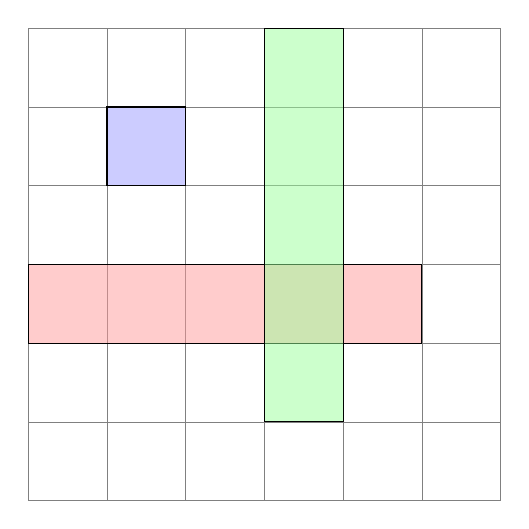
\begin{tikzpicture}
\draw[step=1cm,gray,very thin] (0,0) grid (6,6);
\fill[red!40!white, draw=black, fill opacity=0.5] (0,2) rectangle (5,3);
\fill[green!40!white, draw=black, fill opacity=0.5] (3,6) rectangle (4,1);
\fill[blue!40!white, draw=black, fill opacity=0.5] (1,4) rectangle (2,5);
\end{tikzpicture}
\end{center}

\item Since $\dim(\text{span}\{\phi_a\}_{a \in A}) \leq \abs{A} < \abs{I} = \dim(\mathbb{R}^I)$,  $\{\phi_a\}_{a \in A}$ cannot span $I$. Hence, it is not a basis or a frame.

\item For $u,v \in A$ s.t. $u \neq v$. If $\phi_u \perp \phi_v$
\[\innerprod{\phi_{u}}{phi_{v}} = \sum_{i \in I} \phi_{u}[i] \phi_ {v}[i] = \abs{E_u \bigcap E_v} = \lambda\delta_{u,v} = \begin{cases}
1, & u=v\\
0, & \text{else}
\end{cases} = 0 \qquad(u \neq v)\]
It means that $E_u \bigcap E_v = \emptyset$. For example, in the sample figure in part (a), the blue tile is orthogonal with the red and the green tiles, but the red and green are not orthogonal.

\item Since $\{\phi_a\}_{a \in A}$ are orthogonal, the best approximation of $x$ is its projection on the space spanned by normalized $\{\phi_a\}_{a \in A}$, i.e.
\[\hat{x} = \sum_{a \in A} \frac{\innerprod{x}{\phi_a}}{\norm{\Phi_a}^2} \phi_a.\]

\item If $\{\phi_a\}_{a \in A}$ are not orthogonal, we can construct the corresponding set orthogonal bases using Gram-Schmidt algorithm and project $x$ on it.

\end{enumerate}
	\section{Some DFT Properties}\label{sec:p5}

\begin{enumerate}[(a)]
%----------------------------------------------------------------------------------------------
\item Define $k \bmod N$ as $\langle k \rangle_N$, i.e.
\[\langle k + N \rangle_N = \langle k \rangle_N.\]

The DFT of $x[n]$ is defined as
\[X[k] = \sum_{n=0}^{N-1} x[n] W_N^{-kn}\]
where
\[W_N = e^{j\frac{2\pi}{N}} = \cos(2\pi/N) + j\sin(2\pi /N).\]
Assume that $k = lN+r \Leftrightarrow \langle k \rangle_N = r$, then
\begin{align*}
	W_N^k
	&= \exp(j \frac{2\pi}{N} (lN+r)) \\
	&= \exp(j \frac{2\pi}{N} lN) \exp(j \frac{2\pi}{N} r) \\
	&= 1 \exp(j \frac{2\pi}{N} r) \\
	&= W_N^r = W_N^{\langle k \rangle_N}.
\end{align*}
Similarly, $W_N^{mk} = W_N^{m \langle k \rangle_N}$.

Furthermore, 
\begin{align*}
	X[k]
	&= \sum_{n=0}^{N-1}x[n] W_N^{-n(lN+r)} \\
	&= \sum_{n=0}^{N-1} x[n] W_N^{-nlN} W_N^{-nr} \\
	&= \sum_{n=0}^{N-1} x[n] W_N^{-nr} \\
	&= X[r] = X[\langle k \rangle_N].
\end{align*}

Therefore,
\begin{align*}
	DFT(x[\langle -n \rangle_N])
	&= \sum_{n=0}^{N-1}x[\langle -n \rangle_N] W_N^{-nk} \\
	&= \sum_{m=0}^{N-1} x[m] W_N^{-\langle -m\rangle_N k} \\
	&= \sum_{m=0}^{N-1} x[m] W_N^{mk} \\
	&= X[-k] \\
	&= X[\langle -k \rangle_N].
\end{align*}

%----------------------------------------------------------------------------------------------
\item The circular convolution between $x$ and $y$ can be defined as
\begin{align*}
	(x \circledast y)[n] 
	&= \sum_{m=0}^{N-1} x[m] y[\langle n - m\rangle_N].
\end{align*}
Therefore
\begin{align*}
	DFT((x \circledast y)[n])
	&= \sum_{n=0}^{N-1} \sum_{m=0}^{N-1} x[m] y[\langle n-m\rangle_N] W_N^{-nk} \\
	&= \sum_{m=0}^{N-1} x[m] \sum_{n=0}^{N-1} y[\langle n-m \rangle_N]W_N^{-nk} \\
	&= \sum_{m=0}^{N-1} x[m] W_N^{-mk} Y[k] \\
	&= Y[k] \sum_{m=0}^{N-1} x[m] W_N^{-nk} \\
	&= Y[k] X[k]
\end{align*}

%----------------------------------------------------------------------------------------------
\item The inverse DFT is defined as
\[x[n] = \frac{1}{N} \sum_{k=0}^{N-1} X[k] W_N^{kn}\]
Therefore
\begin{align*}
	IDFT((X \circledast Y)[n])
	&= \frac{1}{N} \sum_{k=0}^{N-1} (X \circledast Y)[k] W_N^{kn} \\
	&= \frac{1}{N} \sum_{k=0}^{N-1} \left( X[m] Y[\langle k - m \rangle_N]\right) W_N^{kn} \\
	&= \frac{1}{N} \sum_{k=0}^{N-1} \left( X[m] Y[\langle k - m \rangle_N]\right) W_N^{mn} W_N^{(k-m)n} \\
	&= \frac{1}{N} \sum_{m=0}^{N-1} X[m]W_N^{mn} \sum_{k=0}^{N-1}Y[\langle k-m \rangle_N] W_N^{(k-m)n} \\
	&= x[n]y[n].
\end{align*}

%----------------------------------------------------------------------------------------------
\item If $x[n]$ is real,
\begin{align*}
	&\Rightarrow x[n] = x^*[n] \\
	&\Rightarrow DFT(x[n]) = DFT(x^*[n]) \\
	&\Rightarrow X[k] = X^*[\langle -k \rangle_N].
\end{align*}

If $x[n]$ is also symmetric,
\begin{align*}
	&\Rightarrow x[n] = x[\langle -n \rangle_N] \\
	&\Rightarrow DFT(x[n]) = DFT(x[\langle -n \rangle_N]) \\
	&\Rightarrow X[k] = X[\langle -k \rangle_N].
\end{align*}

Therefore
\[X[k] = X^*[\langle -k \rangle_N] = X[\langle -k \rangle_N].\]
Hence, $X[k]$ is real (and also symmetric.)

%----------------------------------------------------------------------------------------------
\item If $x[n]$ is symmetric (and real),
\begin{align*}
&\Rightarrow x[n] = -x[\langle -n \rangle_N] \\
&\Rightarrow DFT(x[n]) = -DFT(x[\langle -n \rangle_N]) \\
&\Rightarrow X[k] = -X[\langle -k \rangle_N].
\end{align*}

Therefore
\[X[k] = X^*[\langle -k \rangle_N] = -X[\langle -k \rangle_N].\]
Hence, $X[k]$ is imaginary.
\end{enumerate}

\end{document}